\documentclass[12pt]{article}

\usepackage[utf8]{inputenc}
\usepackage[T1]{fontenc}
\usepackage{amsmath}
\usepackage{amssymb}
\usepackage{graphicx}
\usepackage{booktabs}
\usepackage{hyperref}
\usepackage[round]{natbib}
\usepackage[margin=1in]{geometry}
\usepackage{enumitem}
\usepackage{tikz}
\usetikzlibrary{arrows.meta, positioning, calc}

\title{The Elixir Problem: A Systematic Review of Hoarding-Related Behaviors in Digital Games}
\author{Jiyeon Yoon\\
Independent Researcher\\
\texttt{heznpc@gmail.com}}
\date{}

\begin{document}

\maketitle

\noindent\textbf{Target journal:} \textit{Games and Culture} (SAGE)

\noindent\textbf{Word count:} \textasciitilde{}8,500 (excluding references)

\begin{abstract}
Players routinely finish role-playing games with inventories full of unused potions. They spend hundreds of dollars chasing a complete gacha character roster. They maintain elaborate storage systems across multiple accounts rather than discard a single item. They accumulate libraries of hundreds of unplayed games during digital sales. These behaviors share core psychological mechanisms with clinical hoarding disorder---loss aversion, emotional attachment, decision avoidance, and acquisition-driven positive affect---yet the relevant evidence is scattered across behavioral economics, game studies, gambling research, consumer psychology, and human--computer interaction. No prior review has unified this evidence under a hoarding framework. This paper presents a PRISMA systematic review of PubMed-indexed literature examining hoarding-related behaviors across five game domains: consumable hoarding, gacha/loot box collection, inventory paralysis, completionism, and backlog accumulation. From 227 records identified, 156 met eligibility criteria after screening. The evidence landscape is strikingly uneven: the gacha/loot box domain accounts for 97 eligible papers with strong evidence linking spending to problem gambling and OCD/hoarding symptomatology, while consumable hoarding and backlog accumulation each returned zero eligible papers, representing complete evidence voids. We map the available evidence onto DSM-5 hoarding disorder criteria and the Frost--Hartl cognitive-behavioral model, propose a five-domain theoretical framework distinguishing three PRIMARY domains (gacha/loot box, inventory paralysis, completionism) from two EXPLORATORY domains (consumable hoarding, backlog accumulation), and identify six specific over-pathologization risks that constrain interpretation. This review provides the first unified framework connecting in-game accumulation behaviors to clinical hoarding constructs and proposes a Game Hoarding Inventory as a direction for future psychometric development.
\end{abstract}

\noindent\textbf{Keywords:} hoarding, video games, loot boxes, gacha, loss aversion, systematic review, game design, virtual possessions

\section{Introduction}

A player reaches the final boss of \textit{Final Fantasy VI} with 99 Megalixirs in inventory---items that fully restore the entire party's health and magic---and defeats the boss without using a single one. The behavior is so widespread that Japanese gaming culture has given it a name: \textit{rasuto erikusaa shoukougun} (Last Elixir Syndrome). English-speaking communities call it the ``too good to use'' problem. Korean players recognize it immediately. The pattern transcends language and platform: players hoard consumable items throughout an entire game, ostensibly saving them for a moment of need that never arrives.

This is one instance of a broader behavioral pattern. Gacha and loot box players spend substantial sums pursuing complete character rosters, in patterns associated with fear of missing limited-time offerings and compulsive set-completion urges \citep{Zendle2023, Shibuya2019}. MMORPG players maintain elaborate inventory systems, create alternate characters solely for storage, and purchase additional digital storage space rather than discard items with personal significance \citep{Watkins2012}. Achievement hunters return to games they did not enjoy to pursue 100\% completion \citep{Kruse2016}. Digital storefront users accumulate libraries of hundreds of unplayed games during seasonal sales events.

These behaviors share documented psychological mechanisms with hoarding disorder as characterized in the DSM-5 \citep{APA2013} and the Frost--Hartl cognitive-behavioral model \citep{Frost1996}: loss aversion that makes consumption or discarding feel like a loss, emotional attachment to possessions that extends the self, behavioral avoidance of the distress associated with discarding decisions, and erroneous beliefs about future need or item value. Yet the evidence documenting these mechanisms is scattered. Loss aversion in games appears in behavioral economics and CHI venues. Gacha and loot box research concentrates in gambling studies and addiction journals. Inventory attachment surfaces in consumer behavior research. Completionism is discussed in player motivation taxonomies. Backlog accumulation exists primarily in game design journalism. No prior review has organized these scattered findings under a unified framework.

This paper presents the first systematic review connecting in-game accumulation behaviors to clinical hoarding constructs. We conduct a PRISMA systematic review of PubMed-indexed literature, map findings across five behavioral domains, apply the Frost--Hartl CBT model and DSM-5 hoarding criteria to game contexts, and identify where evidence exists, where it is absent, and where the boundaries of pathology remain contested.

We note at the outset that the eponymous `elixir problem'---consumable hoarding in RPGs---represents one of the review's most striking findings: despite robust documentation in game design practitioner literature and widespread recognition among players across cultures, our systematic search returned zero peer-reviewed empirical studies directly measuring this behavior. This absence is itself a key contribution of the review, identifying consumable hoarding as a domain requiring foundational empirical work. The `elixir problem' serves as the paper's motivating example and organizing metaphor, not its best-evidenced domain.

A necessary caveat at the outset: this paper does \textit{not} argue that in-game hoarding-related behavior constitutes hoarding disorder. It argues that shared psychological mechanisms have been documented in scattered literatures, that these mechanisms have never been systematically organized, and that the relationship between in-game accumulation behavior and clinical hoarding is an empirical question requiring future investigation---not a foregone conclusion. Most in-game item retention is normatively rational behavior within the designed systems of the game. We adopt a dimensional rather than categorical perspective, acknowledging that only extreme manifestations involving genuine distress or functional impairment warrant clinical attention.

\section{The Elixir Problem}

\subsection{Definition and Cross-Cultural Recognition}

The ``elixir problem'' refers to the tendency to accumulate consumable items in games---potions, elixirs, rare ammunition, single-use abilities---and never use them. The term originates from the Megalixir in the \textit{Final Fantasy} series, a powerful full-party restoration item that players infamously save throughout the game and never deploy. The phenomenon is recognized across gaming cultures: English-language communities use ``too good to use syndrome''; Japanese gaming discourse refers to it as \textit{rasuto erikusaa shoukougun} (Last Elixir Syndrome); Korean players recognize the same behavioral pattern in their own terminology. The cross-cultural recognition suggests a behavioral regularity grounded in shared cognitive mechanisms rather than culture-specific norms.

\subsection{Psychological Mechanisms}

Several documented psychological mechanisms converge on the elixir problem:

\textbf{Loss aversion.} \citet{Phillips2020} conducted the only controlled experimental study of loss aversion in a commercial-style video game context, finding that players in a Zelda-style adventure game exhibited strong loss aversion bias across 18 decision points involving gold wagers at varying win-to-loss ratios, despite the temporary and digital nature of the game world. Using a consumable item converts a possessed resource into an expended one---a loss in prospect-theoretic terms \citep{Kahneman1979}. The subjective cost of using an item may exceed the subjective benefit of the effect it produces.

\textbf{Endowment effect.} Once an item occupies inventory space, its subjective value increases by virtue of possession alone. \citet{Krauss2025} found in a 21-paper systematic review that psychological ownership of virtual objects operates through the same three routes as physical ownership: control, identity transfer, and intimate knowledge. \citet{Toh2021} mapped endowment effect and sunk cost mechanisms onto video game decision-making, noting that items acquired through effort (boss drops, quest rewards) are harder to use or discard than vendor-purchased items.

\textbf{Decision avoidance.} Using a consumable requires deciding that \textit{this} is the optimal moment---a determination that is easier to defer indefinitely. Schwartz's \citeyearpar{Schwartz2004} ``maximizer'' profile---seeking the provably best option before committing---maps directly to players who cannot identify the ``right'' moment to use an elixir. The result is permanent deferral: the item is never used because no moment feels sufficiently optimal.

\textbf{Scarcity psychology.} The Japanese cultural concept of \textit{mottainai} (wastefulness aversion) has been explicitly connected to the Last Elixir Syndrome in Japanese game culture discourse (Pixiv Dictionary; MAROGAMES), though not yet in academic literature. The perceived irreplaceability of rare items amplifies reluctance to consume them, even when the game provides no further challenges that would justify saving them.

\textbf{Evidence strength for this domain is moderate.} \citet{Phillips2020} provides experimental evidence for loss aversion in games. \citet{Toh2021} and \citet{Engelstein2020} provide theoretical behavioral economics analyses. However, no study has directly measured the prevalence of consumable hoarding behavior, its psychological correlates, or its relationship to clinical hoarding constructs. The phenomenon is robustly documented in game design practitioner literature (Bycer, multiple Game Wisdom articles; Gamasutra/Game Developer articles) but academically understudied.

\section{Method}

\subsection{Protocol and Registration}

This systematic review follows the Preferred Reporting Items for Systematic Reviews and Meta-Analyses (PRISMA) guidelines \citep{Page2021}. The protocol was developed for PROSPERO pre-registration prior to search execution.

\subsection{Database and Search Strategy}

The primary search was conducted in PubMed. Two complementary queries were executed:

\textbf{Query 1 (broad):}

\begin{verbatim}
(hoard* OR collect* OR "loss aversion" OR "endowment effect"
OR "sunk cost" OR "compulsive buying" OR "compulsive acquisition"
OR "item retention" OR "inventory management"
OR "completionism" OR "achievement hunting"
OR "digital possession*")
AND
(game* OR "video game" OR "virtual" OR "loot box" OR "gacha"
OR "inventory" OR "digital possession" OR "virtual item*"
OR "microtransaction*" OR "backlog")
\end{verbatim}

\textbf{Query 2 (targeted):} A narrower formulation targeting hoarding-specific constructs in game contexts. Query 2 returned 75 results, all of which were duplicates of Query 1 results. The combined yield was 227 unique records.

\subsection{Inclusion and Exclusion Criteria}

\textbf{Inclusion criteria.} (1) Peer-reviewed empirical studies (quantitative, qualitative, or mixed methods), systematic reviews, or meta-analyses. (2) Published in English or Japanese. (3) Studies examining any of: in-game item retention, virtual item hoarding, loot box or gacha collecting behavior, inventory management behavior, game completionism or achievement hunting, game backlog accumulation, psychological ownership of virtual game items, or loss aversion in game contexts. (4) Studies connecting game behavior to hoarding, OCD, compulsive buying, loss aversion, or collecting constructs. (5) No date restriction on publication year.

\textbf{Exclusion criteria.} (1) Non-peer-reviewed sources (grey literature, conference abstracts without full papers, game design practitioner articles). (2) Studies examining digital hoarding (emails, files, photos) without a game component. (3) Studies examining gambling without a game mechanic component (pure gambling studies with no loot box or gacha connection). (4) Editorials, commentaries, and opinion pieces without original data. (5) Studies focused exclusively on game monetization economics without behavioral or psychological measures.

\subsection{Screening Process}

Title and abstract screening was conducted on all 227 unique records using a single rule-based keyword heuristic (\texttt{experiments/src/screening.py}; 1{,}204 lines, standard-library Python), not by two independent human reviewers as PRISMA-2020 recommends. Each paper was classified into one of three categories: Include (clearly relevant to at least one of the five behavioral domains), Maybe (tangentially relevant or requiring full-text review to determine eligibility), or Exclude (clearly outside scope). Papers were coded against six domains: (D1) loss aversion in games, (D2) consumable hoarding, (D3) gacha/loot box, (D4) inventory/virtual possession, (D5) completionism, and (D6) backlog accumulation, plus a cross-domain hoarding link category. The single-screener design and its implications are discussed in the Limitations section; a computer-assisted reproducibility audit using a large language model as a second screener is reported in supplementary materials and is framed as an inter-rater reliability check, not as PRISMA-2020 dual-reviewer screening.

\subsection{Quality Assessment}

Quality assessment tools were applied by study type: the Cochrane Risk of Bias tool (RoB 2) for randomized controlled trials, the Newcastle--Ottawa Scale (NOS) for observational studies, the Critical Appraisal Skills Programme (CASP) qualitative checklist for qualitative studies, AMSTAR 2 for systematic reviews and meta-analyses, and the Joanna Briggs Institute (JBI) checklist for case reports. Each study was rated as high, moderate, or low quality. Quality ratings informed the weighting of conclusions in the narrative synthesis.

Quality assessment was conducted for all 102 included papers. Given the heterogeneity of study designs, results are summarized by domain:

\textbf{Gacha/Loot Box domain (97 papers):} The majority of studies employed cross-sectional survey designs. Of the survey studies assessed using the Newcastle--Ottawa Scale (adapted for cross-sectional designs), approximately 60\% received moderate quality ratings (5--6 stars out of 9), with common limitations including convenience sampling (predominantly university students), self-report measures, and cross-sectional design precluding causal inference. The systematic reviews by \citet{Spicer2022} and related meta-analyses received high AMSTAR 2 ratings. The longitudinal studies \citep{Shibuya2019, Zendle2023b} were rated as moderate-to-high quality. The single case report \citep{Inaguma2024} was rated using JBI criteria as adequate for illustrative purposes but not generalizable.

\textbf{Inventory Paralysis domain (20 papers):} Predominantly qualitative studies assessed using CASP. \citet{Watkins2012} and \citet{Koles2025} received high quality ratings for methodological rigor and thick description. Survey studies \citep{Koklic2025} received moderate ratings.

\textbf{Completionism domain (5 papers):} Primarily motivation taxonomy studies with large samples \citep[n=30,000]{Yee2006}; \citep[n=3,818]{Demetrovics2011}. Rated moderate-to-high for their primary purpose (motivation measurement) but not designed to assess hoarding-like behavior specifically.

\textbf{Exploratory domains (Consumable Hoarding, Backlog):} No papers to assess.

\textbf{Cross-domain (Hoarding Link, 34 papers):} Quality varied widely; clinical hoarding measures (SI-R, OCI-R) used in these studies have established psychometric properties, but their application to game contexts has not been separately validated.

Overall, the evidence base is characterized by: (a) reliance on cross-sectional designs, (b) convenience sampling, (c) geographic concentration in North America and East Asia, and (d) the absence of randomized controlled trials testing causal mechanisms.

\subsection{PRISMA Flow Results}

\begin{figure}[htbp]
\centering
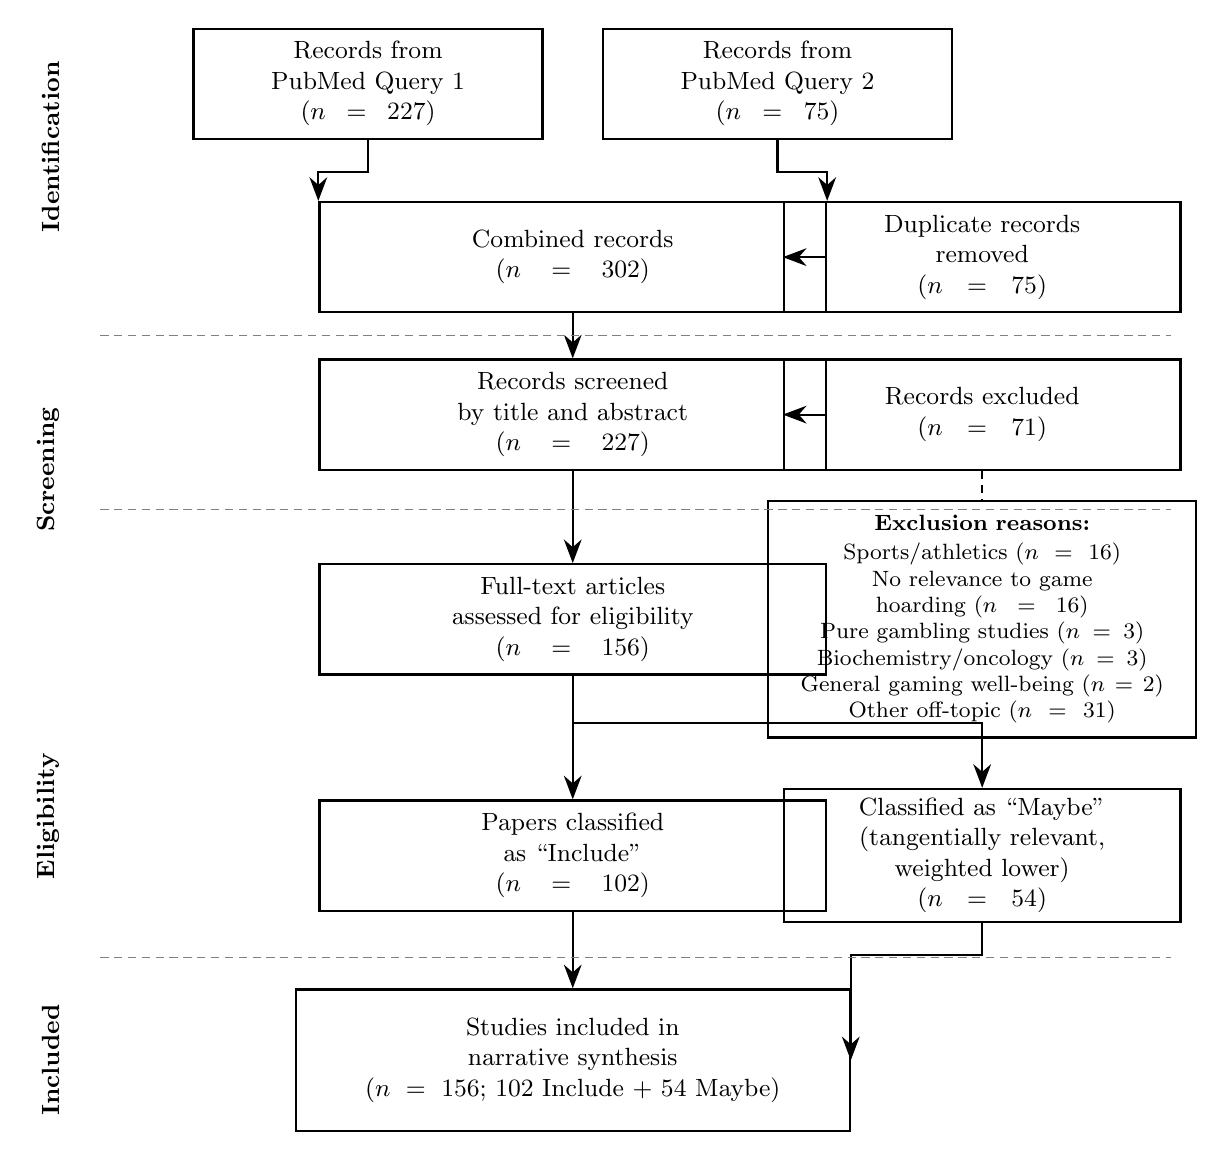
\begin{tikzpicture}[
    box/.style={
        rectangle, draw=black, thick,
        text width=42mm, minimum height=14mm,
        align=center, font=\small
    },
    widebox/.style={
        rectangle, draw=black, thick,
        text width=62mm, minimum height=14mm,
        align=center, font=\small
    },
    sidebox/.style={
        rectangle, draw=black, thick,
        text width=48mm, minimum height=14mm,
        align=center, font=\small
    },
    phaselabel/.style={
        rotate=90, anchor=south, font=\small\bfseries
    },
    arrow/.style={-{Stealth[length=3mm]}, thick},
    node distance=12mm and 18mm
]

% --- Phase labels (left side) ---
\node[phaselabel] at (-5.8, 0.8) {Identification};
\node[phaselabel] at (-5.8, -3.3) {Screening};
\node[phaselabel] at (-5.8, -7.7) {Eligibility};
\node[phaselabel] at (-5.8, -10.8) {Included};

% --- IDENTIFICATION ---
\node[box] (q1) at (-2, 1.6)
    {Records from\\PubMed Query~1\\($n = 227$)};
\node[box] (q2) at (3.2, 1.6)
    {Records from\\PubMed Query~2\\($n = 75$)};
\node[widebox] (combined) at (0.6, -0.6)
    {Combined records\\($n = 302$)};

\draw[arrow] (q1.south) -- ++(0,-0.4) -| (combined.north west);
\draw[arrow] (q2.south) -- ++(0,-0.4) -| (combined.north east);

% --- Duplicates removed ---
\node[sidebox] (dupes) at (5.8, -0.6)
    {Duplicate records\\removed\\($n = 75$)};
\draw[arrow] (combined.east) -- (dupes.west);

% --- SCREENING ---
\node[widebox] (screened) at (0.6, -2.6)
    {Records screened\\by title and abstract\\($n = 227$)};
\draw[arrow] (combined.south) -- (screened.north);

\node[sidebox] (excluded) at (5.8, -2.6)
    {Records excluded\\($n = 71$)};
\draw[arrow] (screened.east) -- (excluded.west);

% --- Exclusion reasons ---
\node[sidebox, text width=52mm, minimum height=30mm, font=\footnotesize] (reasons) at (5.8, -5.2)
    {\textbf{Exclusion reasons:}\\[1pt]
    Sports/athletics ($n = 16$)\\
    No relevance to game\\hoarding ($n = 16$)\\
    Pure gambling studies ($n = 3$)\\
    Biochemistry/oncology ($n = 3$)\\
    General gaming well-being ($n = 2$)\\
    Other off-topic ($n = 31$)};
\draw[thick, densely dashed] (excluded.south) -- (reasons.north);

% --- ELIGIBILITY ---
\node[widebox] (eligible) at (0.6, -5.2)
    {Full-text articles\\assessed for eligibility\\($n = 156$)};
\draw[arrow] (screened.south) -- (eligible.north);

% --- Maybe classification ---
\node[sidebox] (maybe) at (5.8, -8.2)
    {Classified as ``Maybe''\\(tangentially relevant,\\weighted lower)\\($n = 54$)};
\draw[arrow] (eligible.south) -- ++(0,-0.6) -| (maybe.north);

% Redirect to included
\node[widebox] (reviewtype) at (0.6, -8.2)
    {Papers classified\\as ``Include''\\($n = 102$)};
\draw[arrow] (eligible.south) -- (reviewtype.north);

% --- INCLUDED ---
\node[widebox, minimum height=18mm, text width=68mm] (included) at (0.6, -10.8)
    {Studies included in\\narrative synthesis\\($n = 156$; 102 Include $+$ 54 Maybe)};
\draw[arrow] (reviewtype.south) -- (included.north);
\draw[arrow] (maybe.south) -- ++(0,-0.4) -| (included.east);

% --- Dashed phase separators ---
\draw[gray, densely dashed] (-5.4, -1.6) -- (8.2, -1.6);
\draw[gray, densely dashed] (-5.4, -3.8) -- (8.2, -3.8);
\draw[gray, densely dashed] (-5.4, -9.5) -- (8.2, -9.5);

\end{tikzpicture}
\caption{PRISMA flow diagram of study identification, screening, and inclusion. PubMed was the sole bibliographic database searched. Query~2 results were fully duplicated within Query~1, yielding 227 unique records. Of 156 eligible records, 54 were classified as ``Maybe'' (tangentially relevant) and retained with lower weighting in the narrative synthesis.}
\label{fig:prisma}
\end{figure}

\textbf{Identification:} 227 records identified through PubMed search (Query 1: 227 hits; Query 2: 75 hits; 75 duplicates removed).

\textbf{Screening:} 227 records screened by title and abstract.

\textbf{Excluded at screening:} 71 records. Primary exclusion reasons: sports/athletics papers ($n = 16$), no clear relevance to in-game collecting or hoarding behaviors ($n = 16$), pure gambling studies without game mechanic connection ($n = 3$), biochemistry/oncology papers ($n = 3$), general gaming well-being studies without collecting/hoarding angle ($n = 2$), and various off-topic domains including labor economics, patent systems, public health, auction/bidding experiments, and ecology (remaining $n = 31$).

\textbf{Eligible for synthesis:} 156 records (102 Include $+$ 54 Maybe).

Of the 54 papers classified as `Maybe' (tangentially relevant, requiring full-text review for definitive classification), we adopted a conservative approach: these papers were retained in the eligible pool for domain classification and are reported in the domain counts, but were weighted lower in the narrative synthesis. The `Maybe' classification was typically assigned to papers studying game-related behaviors (e.g., purchasing, engagement, monetization) that did not explicitly invoke hoarding, collecting, or retention constructs but whose findings could inform the hoarding framework. A definitive include/exclude decision for these papers requires full-text review, which we flag as a necessary step for the final publication-ready version of this review.

\textbf{Domain distribution of eligible papers:}

\begin{table}[ht]
\centering
\caption{Domain distribution of eligible papers.}
\begin{tabular}{lccc}
\toprule
Domain & Include & Maybe & Total \\
\midrule
D1: Loss Aversion in Games & 4 & 2 & 6 \\
D2: Consumable Hoarding & 0 & 0 & 0 \\
D3: Gacha / Loot Box & 91 & 6 & 97 \\
D4: Inventory / Virtual Possession & 17 & 3 & 20 \\
D5: Completionism & 2 & 3 & 5 \\
D6: Backlog Accumulation & 0 & 0 & 0 \\
Cross-domain: Hoarding Link & 4 & 30 & 34 \\
\bottomrule
\end{tabular}
\end{table}

\textbf{Temporal concentration:} 127 of 156 eligible papers (81.4\%) were published in 2020 or later, reflecting the rapid growth of academic interest in game monetization and behavioral consequences.

\subsection{Synthesis Method}

Narrative synthesis was organized by the five-domain framework. Quantitative meta-analysis was not conducted due to heterogeneity in study designs, populations, measures, and constructs across domains. Even within the gacha/loot box domain, the largest evidence cluster, heterogeneity in outcome measures (problem gambling severity, spending amounts, risky engagement indices) precluded meaningful pooling. Findings are mapped to the Frost--Hartl CBT model components and DSM-5 hoarding disorder criteria in the theoretical framework section.

\section{Results: Evidence by Domain}

\subsection{Loss Aversion in Games (Cross-Cutting Mechanism)}

\textbf{Paper count:} 6 eligible (4 Include, 2 Maybe). \textbf{Evidence strength:} Moderate.

Loss aversion---the tendency to weigh losses more heavily than equivalent gains \citep{Kahneman1979}---functions as a cross-cutting mechanism relevant to all five behavioral domains rather than constituting a domain of its own. The available evidence primarily examines how loss-framed mechanics influence player engagement and decision-making.

\begin{table}[ht]
\centering
\caption{Loss Aversion in Games: Key Evidence.}
\small
\begin{tabular}{p{3.2cm}p{3cm}p{1.5cm}p{6cm}}
\toprule
Author (Year) & Method & N & Key Finding \\
\midrule
Phillips et al.\ (2020) & Experiment (Zelda-style game) & -- & Strong loss aversion across 18 decision points despite virtual, temporary stakes \\
Hong (2023) & Neuroimaging & -- & Reduced loss aversion in value-based decision-making among IGD patients mirrors substance use disorders \\
Anderson (2018) & Observational (chess) & 133M games & Players exert effort to set new personal best ratings and quit once achieved; goal-setting drives persistence \\
Strojny (2026) & Empirical & -- & Sunk-cost effects, gaming-contingent self-worth, and loss aversion persist after initial gratification fades \\
Wang (2020) & Modeling & -- & Dual-system model explains adolescents' excessive gaming through imbalance between impulsive and reflective systems \\
\bottomrule
\end{tabular}
\end{table}

The evidence establishes that loss aversion operates in game contexts, but significant gaps remain. No study has used behavioral economics paradigms (e.g., prospect theory tasks) to measure loss aversion in game resource decisions specifically. No research examines how loss-framed game mechanics---expiring rewards, daily login bonuses, streak systems---exploit loss aversion. The connection between measured loss aversion and specific in-game behaviors such as consumable hoarding or inventory paralysis remains unexplored.

A methodological complication arises from the loss aversion replication literature: a 2022 study reported that loss aversion did not appear for losses under approximately \$40 \citep{Mrkva2020}. Because virtual game items frequently have zero real-world monetary value, the applicability of loss aversion findings from economic contexts to game contexts requires empirical validation rather than assumption.

\subsection{Consumable Hoarding (EXPLORATORY---0 Papers)}

\textbf{Paper count:} 0 eligible. \textbf{Evidence strength:} No peer-reviewed evidence.

The systematic search returned zero PubMed-indexed papers examining consumable hoarding in games. This represents a complete evidence void for the phenomenon that motivates the paper's title.

This absence is notable for two reasons. First, consumable hoarding is extensively documented in game design practitioner literature: Bycer's ``Combating the Hoarding Syndrome in Game Design'' and ``How Hoarding Encourages Bad Game Design'' (Game Wisdom); ``Avoiding the Hoarder Trap in Game Design'' (Gamasutra/Game Developer); BantArcade's ``The Elixir Problem---How to Encourage Players to Use Their Potions''; and TV Tropes' extensive documentation under ``Too Awesome to Use.'' Japanese game culture sources document the phenomenon under the \textit{Last Elixir Syndrome} label (Pixiv Dictionary, MAROGAMES). Second, the indirect academic evidence supporting the underlying mechanisms is moderate: \citet{Phillips2020} demonstrates loss aversion in a game context, \citet{Toh2021} maps behavioral economics constructs to game decisions, and \citet{Engelstein2020} provides a book-length treatment through MIT Press.

The evidence gap is not a gap in the phenomenon itself but a gap in academic attention. The behavior is widely recognized, extensively discussed in design communities, and theoretically grounded in well-established psychological mechanisms. What is missing is any empirical measurement of its prevalence, correlates, individual differences, or relationship to hoarding symptomatology. This domain requires foundational empirical work: prevalence studies, behavioral measurement paradigms, and psychometric development.

\textbf{OpenAlex broader-database check (supplementary).} A pre-registered one-sided extension of the search to the OpenAlex Works API (\texttt{experiments/openalex\_extension/}) returned 200 hits for a D2-targeted query (consumable hoarding / potion hoarding / elixir / too good to use / item retention / resource hoarding, combined with game-context terms). After deduplication against the PubMed corpus and heuristic screening, 6 records were heuristic-Include. Of these, 5 were a single non-game AI containment paper (Q-SLICE CCCE) duplicated as separate Zenodo records, plus a free-to-play monetization dissertation and a trade-classification paper on virtual goods. A pre-registered three-model LLM re-screening (Opus 4-7, Sonnet 4-6, Haiku 4-5) unanimously excluded all 6, in line with the heuristic's known over-inclusion bias documented in the LLM-second-reviewer audit. The D2 evidence void survives the broader-database check.

\subsection{Gacha/Loot Box (PRIMARY---97 Papers)}

\textbf{Paper count:} 97 eligible (91 Include, 6 Maybe). \textbf{Evidence strength:} Strong.

The gacha/loot box domain constitutes the overwhelming majority of the evidence base, accounting for 62.2\% of all eligible papers. This reflects both the regulatory urgency surrounding randomized monetization mechanics and the relative ease of measuring spending as an outcome variable. The evidence is temporally concentrated: the domain has grown rapidly since approximately 2017, with the majority of studies published after 2020.

\begin{table}[ht]
\centering
\caption{Gacha/Loot Box: Key Evidence.}
\small
\begin{tabular}{p{3.2cm}p{3cm}p{1.5cm}p{6cm}}
\toprule
Author (Year) & Method & N & Key Finding \\
\midrule
Garea et al.\ (2023) & Cross-sectional survey (NZ, AU, US) & 1,049 & OCD and hoarding symptomatology associated with greater loot box spending \\
Spicer et al.\ (2022) & Systematic review and meta-synthesis & 13 pubs & $r = .27$ (loot boxes and problem gambling); $r = .40$ (loot boxes and problem gaming) \\
Tang et al.\ (2022) & Cross-sectional survey, Chinese young adults & 117 & 25\% of gacha gamers at high problem gambling risk; 40\% moderate risk \\
Tang et al.\ (2025) & Cross-sectional survey, Hong Kong young adults & 281 & Gameplay frequency and duration were associated with gambling severity; gacha spending was associated with gambling severity \\
Shibuya et al.\ (2019) & Longitudinal (6-month), Japanese youth & 948 & Exposure to limited-time gacha predicted increased spending 6 months later \\
Drummond et al.\ (2025) & Reanalysis & -- & Loot box spending associated with greater distress when normalized to disposable income \\
Palmer (2025) & Longitudinal & -- & Loot box purchases predict gambling initiation; direct-purchase microtransactions do not \\
Zendle (2025) & Longitudinal (UK compliance) & -- & UK self-regulation achieves 64\% probability disclosure compliance vs.\ South Korea's legally mandated 84\% \\
Lopez-Gonzalez et al.\ (2024) & SEM, Spain & 542 & Problematic loot box use statistically mediates the cross-sectional relationship between IGD and online gambling disorder \\
Inaguma et al.\ (2024) & Clinical case report, Japan & 1 & Gaming disorder case with substantial financial burden from gacha spending \\
Mosconi (2026) & Cross-sectional survey & 6,621 & Convergence between gaming monetization spending and gambling vulnerabilities \\
Sanmartin (2023) & Survey & 475 & 45.5\% reported guilt over loot box purchasing; 50\% reported distress; 17\% reported loss of control \\
\bottomrule
\end{tabular}
\end{table}

\textbf{Study design distribution:} Cross-sectional surveys ($n = 43$), unspecified designs ($n = 35$), longitudinal studies ($n = 9$), systematic reviews and meta-analyses ($n = 4$), scale validation studies ($n = 3$), reviews and commentaries ($n = 3$), experimental studies ($n = 2$), qualitative studies ($n = 2$), and content analyses ($n = 1$).

\textbf{Design-distribution robustness audit (supplementary).} A pre-registered three-model LLM re-classification of the 102 D3-tagged papers (\texttt{experiments/d3\_design\_audit/protocol.md}; Opus 4-7, Sonnet 4-6, Haiku 4-5) reported 90\,\% unanimous and 9\,\% majority three-LLM agreement on study design from title and abstract alone. The load-bearing \emph{longitudinal $n = 9$} claim was confirmed exactly by LLM majority (9 of 9 papers classified longitudinal; 8 of those unanimous across all three models). The \emph{qualitative $n = 2$} claim was also confirmed exactly. Two count claims would shift if the heuristic-derived distribution were replaced by the LLM-majority distribution: \emph{unspecified} would collapse from 35 to 1 (the LLM consensus assigns 34 of the 35 heuristic-``unspecified'' papers to a specific design category), and \emph{reviews and commentaries} would rise from 3 to 13, consistent with the broader finding (reported in the Limitations) that the rule-based heuristic admits commentary and conceptual pieces at a non-trivial rate. The audit is reported as a supplementary descriptive check; the heuristic-derived counts in this paragraph are retained as the primary numbers, with the LLM re-classification recorded in \texttt{experiments/results/d3\_design\_audit\_summary.md}.

Several key findings emerge from the synthesis. First, the gambling--loot box nexus is well established: multiple large-scale surveys and several meta-analyses confirm moderate-to-strong positive correlations between loot box spending and problem gambling severity \citep{Li2019, Zendle2019, Zendle2020, Spicer2022}. Second, psychological mechanisms including impulsivity, fear of missing out, reward sensitivity, and OCD/hoarding symptomatology have been identified as correlates of excessive spending \citep{Garea2023, Biegun2023}. Third, vulnerable populations---adolescents, individuals with pre-existing gambling problems, and those with OCD/hoarding symptoms---appear disproportionately represented among high spenders \citep{Close2023, Charnock2024}. Fourth, validated instruments now exist for measuring risky loot box engagement, including the Risky Loot Box Index \citep{Guo2025, Forsstrom2022}.

\textbf{Methodological concerns.} \citet{Tang2022} modified the Problem Gambling Severity Index by replacing ``gambling'' with ``spending money on gacha mechanics.'' Subsequent commentary argues this creates a novel construct that does not validly measure problem gambling (Frontiers in Psychiatry, 2025). This methodological concern extends to a portion of the gacha-gambling literature that relies on adapted gambling instruments. Additionally, the overwhelming dominance of cross-sectional designs limits causal inference. The nine longitudinal studies provide stronger evidence for temporal precedence \citep{Shibuya2019, Palmer2025, Zendle2023b} but cannot establish causation.

\textbf{Gaps specific to hoarding.} Despite the large evidence base, no study has applied the full DSM-5 hoarding disorder criteria to gacha collection behavior. Research focuses on spending and gambling-adjacent outcomes rather than on the accumulation, retention, and difficulty discarding dimensions that characterize hoarding. The connection between loot box spending and the psychological experience of accumulating, organizing, and retaining in-game items over time remains underexplored.

\subsection{Inventory Paralysis (PRIMARY---20 Papers)}

\textbf{Paper count:} 20 eligible (17 Include, 3 Maybe). \textbf{Evidence strength:} Moderate.

Inventory paralysis refers to the difficulty players experience when managing, organizing, and discarding items in inventory-limited games. In MMORPGs such as \textit{World of Warcraft}, \textit{Final Fantasy XIV}, and \textit{Destiny 2}, players purchase additional storage space, create alternate characters dedicated solely to holding overflow items, and maintain elaborate organizational systems to avoid discarding anything.

\begin{table}[ht]
\centering
\caption{Inventory Paralysis / Virtual Possession: Key Evidence.}
\small
\begin{tabular}{p{3.2cm}p{3cm}p{1.5cm}p{6cm}}
\toprule
Author (Year) & Method & N & Key Finding \\
\midrule
Watkins \& Molesworth (2012) & Qualitative & -- & Players form genuine emotional attachments to ``irreplaceable'' virtual goods; attachment mirrors physical possession attachment \\
Krauss \& Wienrich (2025) & Systematic review (21 papers) & -- & Psychological ownership operates through self-efficacy, self-identity, and belonging motives; control, identity transfer, and intimate knowledge routes \\
Belk (2013) & Theoretical & -- & Extended self incorporates virtual/digital objects through dematerialization, reembodiment, sharing, co-construction, distributed memory \\
Honarvar \& Sepehrinia (2025) & Systematic review (25 papers) & -- & Proposes ``datafication'' as sixth dimension of digital extended self beyond Belk's (2013) five \\
Koles (2025) & Qualitative (20 French players) & 20 & Even cosmetic items offer perceived competitive advantages; collector personas exhibit identity-attachment motives \\
Koklic (2025) & Survey $+$ experiment & 625 $+$ 177 & Psychological ownership positively related to both digital hoarding and digital piracy; collectivism moderates \\
Nicklin et al.\ (2021) & Qualitative & 28 & Digital items within loot boxes can be highly valued; certain motivations disproportionately endorsed by those with gambling symptoms \\
Boffel (2021) & Experimental & -- & Avatar identification positively related to perceived competence and self-estimated performance \\
\bottomrule
\end{tabular}
\end{table}

The evidence establishes that psychological ownership of virtual game items operates through the same mechanisms as physical ownership \citep{Krauss2025}, that players form genuine emotional attachments to virtual possessions \citep{Watkins2012}, and that virtual objects function as extensions of the self \citep{Belk2013, Honarvar2025}.

\textbf{The IKEA effect as a mechanism.} The IKEA effect---the tendency to overvalue items one has personally created or customized \citep{Norton2012}---provides a specific mechanism for inventory attachment beyond general endowment. Players who craft, enhance, or upgrade items invest labor that may inflate subjective value disproportionate to functional utility. This is distinct from mere possession (endowment effect) because it adds a labor-investment dimension particularly relevant to crafting and enhancement systems in RPGs and MMORPGs. A player who spent hours gathering materials and crafting armor will overvalue it relative to a functionally identical vendor-purchased item. This mechanism may help explain why players resist discarding crafted or upgraded items even when superior replacements are available.

\textbf{Critical absence.} Research on inventory paralysis specifically---the decision-making difficulty arising from large item collections, the reluctance to discard, the choice overload from extensive inventories---is absent from the evidence base. While psychological ownership and virtual possession are studied, the behavioral consequences of large inventories remain unexamined. No study has quantitatively measured inventory management time or its relationship to hoarding symptomatology.

\subsection{Completionism (PRIMARY---5 Papers)}

\textbf{Paper count:} 5 eligible (2 Include, 3 Maybe). \textbf{Evidence strength:} Weak.

Completionism---the drive to achieve 100\% completion, collect all items, unlock all achievements, and obtain every available collectible---is a well-recognized player motivation in game design frameworks \citep{Bartle1996, Yee2006} but is sparsely represented in PubMed-indexed literature. The near-absence of dedicated completionism research on PubMed is notable given the extensive game studies literature on player typologies and motivations published in non-medical venues.

\begin{table}[ht]
\centering
\caption{Completionism: Key Evidence (supplemented with non-PubMed sources).}
\small
\begin{tabular}{p{3.2cm}p{3cm}p{1.5cm}p{6cm}}
\toprule
Author (Year) & Method & N & Key Finding \\
\midrule
Yee (2006) & Factor-analytic survey & 30,000 & Achievement component (advancement, mechanics, competition) identified as core player motivation \\
Bartle (1996) & Theoretical taxonomy & -- & Achiever player type defined by accumulating and collecting archetype \\
Demetrovics et al.\ (2011) & Scale development (MOGQ) & 3,818 & Seven-factor gaming motivation model including competition and skill development \\
Ghibellini \& Meier (2025) & Meta-analysis & -- & No memory advantage for unfinished tasks (Zeigarnik effect not supported); behavioral drive to resume interrupted tasks (Ovsiankina effect) supported \\
Kruse (2016) & Survey & -- & Self-described completionists more likely to return to games they did not enjoy to finish achievements \\
\bottomrule
\end{tabular}
\end{table}

\textbf{The Zeigarnik-to-Ovsiankina reframe.} Completionism was previously theorized to operate through the Zeigarnik effect---the idea that unfinished tasks are better remembered, creating intrusive thoughts that drive completion. However, a 2025 meta-analysis \citep{Ghibellini2025} found no reliable memory advantage for unfinished tasks, undermining the Zeigarnik effect as traditionally formulated. Crucially, the same meta-analysis \textit{did} support the Ovsiankina effect: a behavioral drive to resume and complete interrupted tasks, independent of any memory advantage.

This distinction matters for understanding completionism in games. The mechanism is not ``players remember uncompleted achievements more vividly'' but rather ``players experience a behavioral compulsion to resume and finish tasks once started, regardless of whether those tasks are better remembered.'' This reframe strengthens the connection to hoarding: completionism is about compulsive behavioral resumption---an avoidance of the unfinished state---rather than enhanced memory salience. This aligns with the behavioral avoidance component of the Frost--Hartl CBT model.

\textbf{Gaps.} No validated scale specifically measures completionist tendencies in gamers. No study examines when completionism shifts from rewarding engagement to compulsive behavior that would meet hoarding-adjacent criteria. The link between completionism and clinical OCD measures is theorized but not empirically established in a game-specific context.

\subsection{Backlog Accumulation (EXPLORATORY---0 Papers)}

\textbf{Paper count:} 0 eligible. \textbf{Evidence strength:} No peer-reviewed evidence.

Game backlog accumulation---the pattern of purchasing far more games than one plays, sometimes described as the ``pile of shame''---returned zero eligible papers in the systematic search. This represents the second complete evidence void alongside consumable hoarding.

The phenomenon is well-documented outside academic literature. Publicly available platform data (SteamSpy, SteamDB) reveal that many users have libraries containing hundreds of unplayed games. Game design journalism regularly analyzes ``backlog psychology'' drawing on Schwartz's choice paralysis framework, scarcity effects of time-limited sales, and social comparison mechanisms (The Game Crater; Ganker; Odyssey Online).

Indirect academic evidence exists in adjacent literatures. \citet{Frost1998} found that 61\% of clinical hoarders meet compulsive buying criteria, with acquisition associated with positive affect. \citet{Vinoi2024} found that perceived low price has a positive impact on digital hoarding and that discarding difficulty mediates between perceived low price and hoarding behavior. \citet{Hamari2017} identified 10 psychological constructs driving virtual goods purchase in a 24-study meta-analysis.

The absence of dedicated research is itself a finding. The psychology of digital goods accumulation beyond impulse buying is understudied across all digital media, not only games. This domain requires foundational empirical work: prevalence studies, behavioral characterization, and assessment of whether backlog accumulation constitutes a meaningful behavioral pattern or simply reflects rational consumer behavior in the context of aggressive digital pricing strategies.

\textbf{OpenAlex broader-database check (supplementary).} The same pre-registered extension that re-checked D2 also targeted D6 (backlog / pile of shame / unplayed games / Steam library, combined with game-context terms) and returned 200 hits. After deduplication against the PubMed corpus and heuristic screening, 5 records were heuristic-Include. None of them were studies of digital backlog accumulation: they were two duplicate listings of an edited volume on game-development labour (\textit{Game Production Studies}), a 2015 \textit{Journal of Operations Management} paper on supply-chain hoarding (which mentions ``hoarding'' but concerns physical inventory), a study of indie-game value-crafting, and a dissertation on accessibility for disabled gamers. The three-model LLM re-screening unanimously excluded all 5. The D6 evidence void survives the broader-database check.

\section{Cross-Domain Evidence}

\subsection{The Digital--Physical Hoarding Link}

The cross-domain hoarding link category yielded 34 eligible papers (4 Include, 30 Maybe), providing the theoretical bridge between in-game behavior and clinical hoarding constructs. The evidence establishes meaningful connections between digital and physical hoarding but has not yet extended to game-specific hoarding.

\begin{table}[ht]
\centering
\caption{Cross-Domain Evidence.}
\small
\begin{tabular}{p{3.2cm}p{3cm}p{1.5cm}p{6cm}}
\toprule
Author (Year) & Method & N & Key Finding \\
\midrule
Thorpe, Bolster, \& Neave (2019) & Survey & 282 & Physical hoarding and digital hoarding correlated at $r = .55$ ($p < .001$); OCD correlated with digital hoarding at $r = .58$; only OCD and physical hoarding predicted digital hoarding in regression \\
Luxon, Hamilton, Bates, \& Chasson (2019) & Experiment (Pinterest users) & 101 & Electronic object attachment mediated relationship between hoarding severity and distress when asked to discard electronic possessions \\
Neave et al.\ (2019) & Scale development (2 samples) & -- & Digital Hoarding Questionnaire (DHQ): 10-item measure; digital hoarding common, with emails most hoarded category \\
Koklic (2025) & Survey $+$ experiment & 625 $+$ 177 & Psychological ownership positively predicts digital hoarding; collectivism and uncertainty avoidance moderate \\
Garea et al.\ (2023) & Cross-sectional survey & 1,049 & OCD and hoarding symptomatology associated with greater loot box spending---the most direct evidence linking hoarding tendencies to in-game purchasing \\
\bottomrule
\end{tabular}
\end{table}

\citet{Thorpe2019} provides the strongest evidence that digital and physical hoarding share psychological mechanisms ($r = .55$) and that OCD symptomatology predicts both. \citet{Garea2023} extends this by demonstrating that hoarding symptomatology is associated with specific in-game spending behavior.

\subsection{The Untested Transfer Chain}

The evidence suggests a potential transfer chain: \textbf{game hoarding $\rightarrow$ digital hoarding $\rightarrow$ physical hoarding.} \citet{Thorpe2019} establishes the digital--physical link. \citet{Garea2023} establishes the game--hoarding symptomatology link. However, no study has tested whether in-game hoarding behavior (as opposed to general digital hoarding of files and emails) predicts either digital hoarding or physical hoarding. The full transfer chain remains entirely untested. This is the review's most important empirical hypothesis for future research: whether behaviors expressed in game environments are associated with broader digital and physical accumulation patterns.

\section{Theoretical Framework}

\subsection{DSM-5 Mapping}

DSM-5 Hoarding Disorder (300.3) requires persistent difficulty discarding, perceived need to save with distress at discarding, accumulation causing congestion, and clinically significant distress or impairment. We map each criterion onto in-game behavior and assess the available evidence.

\begin{table}[ht]
\centering
\caption{DSM-5 Hoarding Disorder Criteria Applied to Game Contexts.}
\small
\begin{tabular}{p{2.5cm}p{2.5cm}p{3.5cm}p{4.5cm}}
\toprule
DSM-5 Criterion & Physical Hoarding & In-Game Adaptation & Evidence \\
\midrule
1.\ Difficulty discarding & Cannot discard objects & Cannot sell, destroy, or consume items; inventory full, still will not discard & Qualitative: Watkins \& Molesworth (2012). Quantitative: none for games specifically \\
2.\ Perceived need to save; distress at discarding & ``I might need it someday'' & ``I might need this potion for a harder fight''; ``This item might become rare'' & Theoretical: Toh (2021), Engelstein (2020). Experimental: Phillips et al.\ (2020) for loss aversion \\
3.\ Accumulation causing congestion & Cluttered living space & Full inventory, multiple storage characters, paid storage expansions & Anecdotal: extensive forum and community evidence. Academic: none \\
4.\ Clinically significant distress or impairment & Functional impairment in daily life & Time impairment (hours managing inventory), financial impairment (gacha spending), gameplay impairment (unused resources) & Financial: Tang et al.\ (2022), Inaguma (2024), Sanmartin (2023). Time: not measured \\
5.\ Not attributable to medical condition & Brain injury, etc. & Not applicable in game context & N/A \\
6.\ Not better explained by another disorder & OCD, depression & Distinguish from gambling disorder (gacha), Internet Gaming Disorder, normal collecting & Zendle et al.\ (2023): OCD/hoarding linked to loot box spending. Lopez-Gonzalez et al.\ (2024): loot boxes mediate IGD--gambling link \\
\bottomrule
\end{tabular}
\end{table}

The mapping reveals that Criteria 1 and 2 have moderate theoretical and limited empirical support in game contexts; Criterion 3 translates only metaphorically (digital congestion has no physical health consequences); Criterion 4 has evidence for financial impairment (gacha spending) but not for temporal impairment; and Criterion 6 presents significant differential diagnosis challenges given the overlap with gambling disorder and Internet Gaming Disorder.

\subsection{Frost--Hartl CBT Model Applied to Games}

\citet{Frost1996} proposed the most influential cognitive-behavioral model of hoarding, identifying four components. Each maps onto in-game behavior.

\begin{table}[ht]
\centering
\caption{Frost--Hartl CBT Model Components in Game Contexts.}
\small
\begin{tabular}{p{2.8cm}p{4cm}p{6cm}}
\toprule
Frost--Hartl Component & Physical Hoarding Manifestation & In-Game Manifestation \\
\midrule
Information processing deficits & Difficulty categorizing; difficulty deciding what to keep & Inventory paralysis; inability to assess which items are truly needed vs.\ disposable \\
Emotional attachment & Objects as extensions of self; safety and comfort from possessions & Items with personal history (first rare drop, gift from guild member); IKEA effect inflates value of crafted/upgraded items \citep{Norton2012}; avatar identification \citep{Boffel2021} \\
Behavioral avoidance & Avoiding the distress of discarding & Avoiding inventory management entirely; creating overflow storage rather than deciding; Ovsiankina-driven compulsion to finish incomplete sets rather than accept incompleteness \\
Erroneous beliefs about possessions & ``I might need this''; ``It would be wasteful to discard'' & ``I might need this elixir for the final boss''; ``This item might become rare or valuable''; ``I worked hard to get this'' \\
\bottomrule
\end{tabular}
\end{table}

An additional mechanism applies in game contexts that intensifies hoarding beyond what occurs with physical possessions. \citet{Frost1998} found that approximately 85\% of clinical hoarders report excessive acquisition with positive emotional reinforcement. In games, acquisition mechanics---gacha pulls, loot drops, achievement unlocks, sale purchases---are explicitly designed by game developers to maximize positive affect at the moment of acquisition. Game designers have, in effect, optimized the acquisition-pleasure loop far beyond what occurs naturally with physical possessions.

\subsection{The Collecting--Hoarding Boundary}

\citet{Nordsletten2012} articulated criteria for distinguishing collecting from hoarding, which have never been systematically applied to game contexts.

\begin{table}[ht]
\centering
\caption{Collecting vs.\ Hoarding Applied to Game Contexts.}
\small
\begin{tabular}{p{2.5cm}p{2.5cm}p{2.5cm}p{5cm}}
\toprule
Feature & Collectors & Hoarders & In-Game Pattern \\
\midrule
Organization & Organized, curated displays & Chaotic accumulation & Both patterns exist; some players maintain meticulous inventories, others accumulate indiscriminately \\
Emotional valence & Pride, pleasure in the collection & Distress, anxiety about items & Gacha players report both acquisition pleasure and missing-item distress \citep{Sanmartin2023} \\
Trading willingness & Willing to trade, upgrade, or sell & Resist discarding at all costs & Varies by domain; completionists resist removing anything from collection \\
Value congruence & Subjective value aligned with community valuation & Value incongruent with actual worth & ``This level-1 sword has sentimental value'' represents classic incongruent valuation \\
Impairment & Life enriched by collection & Life impaired by accumulation & Time and financial costs cross this line for some players \citep{Tang2022, Inaguma2024} \\
\bottomrule
\end{tabular}
\end{table}

The boundary between collecting and hoarding in games is further complicated by the fact that game design deliberately blurs it. Set-completion mechanics, limited-time exclusives, achievement systems, and rarity tiers are designed to transform collectors into completionists---to shift players from curated, selective engagement toward exhaustive, compulsive acquisition. The clinical boundary identified by \citet{Nordsletten2012} may be actively undermined by design incentives.

\section{Discussion}

\subsection{Evidence Strength Assessment}

The systematic review reveals a dramatically uneven evidence landscape across the five behavioral domains.

\begin{table}[ht]
\centering
\caption{Evidence Strength Summary by Domain.}
\small
\begin{tabular}{p{2.3cm}p{1.8cm}p{1.3cm}p{1.5cm}p{5.5cm}}
\toprule
Domain & Classification & Paper Count & Evidence Strength & Key Finding \\
\midrule
Loss aversion in games & Cross-cutting mechanism & 6 & Moderate & Mechanism established experimentally (Phillips et al., 2020); unreplicated; game-specific applications not tested \\
Consumable hoarding & EXPLORATORY & 0 & None (peer-reviewed) & Complete evidence void; extensive practitioner literature; requires foundational empirical work \\
Gacha/loot box & PRIMARY & 97 & Strong & Multiple large-N studies, systematic reviews, longitudinal evidence; gambling and OCD/hoarding symptomatology links well established \\
Inventory paralysis & PRIMARY & 20 & Moderate & Psychological ownership and emotional attachment established; inventory management behavior not directly measured \\
Completionism & PRIMARY & 5 & Weak & Motivation taxonomies exist; Ovsiankina mechanism supported; no completionism-specific measurement; no pathology boundary tested \\
Backlog accumulation & EXPLORATORY & 0 & None (peer-reviewed) & Complete evidence void; compulsive buying and digital hoarding literature provides indirect theoretical support \\
Cross-domain transfer & Cross-cutting & 34 & Moderate & Digital--physical hoarding link established ($r = .55$); game-specific transfer entirely untested \\
\bottomrule
\end{tabular}
\end{table}

The evidence asymmetry is itself a key finding. The concentration of 97 papers in the gacha/loot box domain against zero papers in consumable hoarding and backlog accumulation reflects where research funding, regulatory urgency, and measurable outcome variables converge. Spending is easy to quantify; the subjective experience of choosing not to use a potion is not. This asymmetry does not indicate that the underrepresented domains are less important---it indicates they are less studied.

\subsection{Over-Pathologization Risks}

The application of a hoarding framework to game behavior carries substantial over-pathologization risks that must be addressed directly. We identify six specific risks:

First, \textbf{most in-game hoarding is normatively rational.} Saving consumables for harder fights is sound strategy when information about future challenges is incomplete. Not all item retention is pathological; much of it reflects sensible resource management under uncertainty. The paper must not frame adaptive behavior as disordered.

Second, \textbf{game designers create the conditions.} Limited inventory space, artificial scarcity, FOMO timers, and set-completion designs are deliberate. When players respond to these incentives in predictable ways, attributing the resulting behavior to individual pathology risks victim-blaming. The behavior may be better understood as a rational response to a designed environment than as a symptom of psychological dysfunction.

Third, \textbf{virtual items have zero physical storage cost.} A central criterion of physical hoarding disorder---cluttered living space that impairs functioning---does not translate directly to digital contexts. ``Congestion'' in games is a design constraint (inventory limits) rather than a health hazard. The functional impairment in game hoarding, if it exists, is temporal and financial rather than spatial.

Fourth, \textbf{cultural framing matters.} Collecting and completionism are socially rewarded in gaming communities. Applying the label ``hoarding'' pathologizes behavior that communities celebrate as dedication, thoroughness, or mastery. The Japanese Last Elixir Syndrome is treated as a humorous shared experience, not a clinical concern. Imposing a disorder framework onto behavior that communities experience as positive risks cultural insensitivity.

Fifth, \textbf{a systematic review risks overstating coherence.} By organizing scattered evidence under a ``hoarding framework,'' this paper imposes a clinical lens that may not be warranted by the evidence. Alternative, non-pathological explanations---rational resource management, social signaling through rare item display, entertainment value of collecting---may be more parsimonious for most instances of the behaviors described.

Sixth, \textbf{the boundary between engagement and pathology is contested.} The over-pathologization debate in gaming research is well-documented. \citet{Aarseth2017} warned of a ``tsunami of false positive referrals'' following the WHO's Gaming Disorder classification. \citet{King2020} found that 56 items across 20 gaming disorder screening tools risk pathologizing normal gaming behavior, including mood changes, desire to play, and immersion. \citet{Bean2017} argued that applying substance use disorder criteria to gaming ``too often pathologizes normal thoughts, feelings and behavior.'' These concerns apply directly to any attempt to frame game hoarding behaviors using clinical constructs.

\textbf{This paper's position} is explicit: it does not argue that in-game hoarding \textit{is} hoarding disorder. It argues that (a) shared psychological mechanisms are documented, (b) for a subset of players, related behaviors are associated with genuine distress and impairment, (c) game design mechanics may engage vulnerabilities associated with hoarding, (d) the evidence base requires systematic organization before empirical claims can be tested, and (e) the relationship between in-game and real-world hoarding is an empirical question for future research.

\subsection{Implications for Game Design}

The framework has practical implications for game designers. Several design solutions documented in practitioner literature directly address the mechanisms identified in this review. Recoverable consumables (such as the Estus Flask system in \textit{Dark Souls}, which replenishes at checkpoints) may mitigate the loss aversion associated with consumable hoarding. Abundant item design may reduce scarcity psychology. Removing or expanding inventory limits may reduce the distress associated with forced discarding. Guaranteed pity systems in gacha mechanics cap the financial cost of set completion. These are not merely quality-of-life improvements; they are interventions targeting specific psychological mechanisms.

Additionally, in-game hoarding severity metrics---unused item counts, inventory fullness ratios, discard rates, time spent in inventory management---could serve as behavioral telemetry markers for player well-being monitoring. Players whose inventory behavior shifts dramatically may be experiencing increased difficulty with discarding decisions, which could warrant prompts or design interventions.

\subsection{Implications for Clinical Practice}

Clinicians should approach these findings with appropriate caution. The evidence does not support screening for ``game hoarding disorder'' as a clinical entity. However, three practice-relevant points emerge. First, gacha spending should be screened alongside gambling behavior, as the evidence for overlap is substantial \citep{LopezGonzalez2024, Spicer2022}. Second, clinicians treating hoarding disorder should consider asking about digital and in-game accumulation behavior \citep{Thorpe2019}. Third, in-game hoarding behavior \textit{may} function as an early, low-stakes indicator of hoarding tendencies---but this remains an empirical hypothesis, not an established finding.

\subsection{Regulatory Context}

The regulatory landscape provides context for the clinical significance of the gacha/loot box domain specifically. Belgium banned paid loot boxes in 2018. The Netherlands classifies paid loot boxes with real-money advancement as unlawful. The European Union's proposed Digital Fairness Act (consultation launched July 2025) includes provisions to ban near-miss animations and require real-currency price display for virtual items. South Korea's probability disclosure law (March 2024) achieves 84\% industry compliance according to Zendle's \citeyearpar{Zendle2025} comparative study. Brazil's Lei Felca (Law 15.211/2025, effective March 2026) prohibits loot boxes in games accessible to minors. Japan banned complete gacha (combination-prize mechanics) in 2012. The United Kingdom and United States lag substantially behind in regulatory action.

The hoarding framework developed here provides additional justification for regulation beyond gambling parallels. Set-completion compulsion, FOMO exploitation, and acquisition-driven affect are exploitable vulnerabilities distinct from gambling mechanisms. Regulation addressing only the gambling dimension of loot boxes may leave hoarding-related vulnerabilities unaddressed.

\subsection{Future Directions}

Three research directions emerge from this review.

\textbf{Game Hoarding Inventory (GHI) development.} The five-domain framework and the mechanistic mapping to Frost--Hartl CBT components provide the conceptual basis for developing a psychometric instrument measuring game-specific hoarding tendencies. Such an instrument would require expert panel item generation (game researchers, clinical psychologists, game designers), exploratory and confirmatory factor analysis on independent samples, and convergent/discriminant validity testing against the Saving Inventory-Revised \citep{Frost2004}, Digital Hoarding Questionnaire \citep{Neave2019}, OCI-R hoarding subscale \citep{Foa2002}, IGDS9-SF \citep{Pontes2015}, and Problem Gambling Severity Index \citep{Ferris2001}.

As a starting point, we provide an 18-item GHI draft (\texttt{experiments/ghi\_face\_validity/items\_v1.json}) covering the three primary domains (4 items each: D3 gacha, D4 inventory paralysis, D5 completionism), the two exploratory domains (2 items each: D2 consumable hoarding, D6 backlog accumulation), and two cross-cutting mechanisms (loss aversion on virtual resources, emotional attachment to functionally-useless items). A pre-registered face-validity audit (\texttt{experiments/ghi\_face\_validity/protocol.md}) applied the \citet{King2020} over-pathologization framework---Scope, Language, and Overpathologizing---using three Claude models (Opus 4-7, Sonnet 4-6, Haiku 4-5) as independent judges, $18 \times 3 \times 3 = 162$ judgments in total. Per the pre-registered decision rule, items flagged on $\geq 6/9$ judgments require revision before any human-subjects work. In v1 four items met this threshold: GHI-01 (consumable saving), GHI-03 (gacha set-completion spending), GHI-15 (sale-driven game purchasing), and GHI-18 (sentimental attachment to virtual items). Their common failure mode was a missing distress, impairment, escalation, or loss-of-control marker, which would otherwise distinguish the described behavior from normal engaged play; one item (GHI-10, refusal to discard crafted items) was under review (3-5/9 flags).

A v2 re-audit (\texttt{items\_v2.json}; same 162-judgment protocol) rewrote those five items with explicit distress, impairment, escalation, or loss-of-control markers and held the remaining thirteen items constant. The five revised items dropped from a combined 25/45 flags in v1 to 0/45 in v2; in v2 \emph{no} item meets the REVISE threshold, one item remains under review (GHI-08, paid-storage workaround), and seventeen are provisionally retained. As a sanity check, no unrevised item showed an absolute flag-count change of $\geq 3$ between v1 and v2, indicating that the LLM-judge baseline is stable enough that the revision-driven drops can be attributed to the item rewrites rather than to judge instability. The v1$\rightarrow$v2 comparison is reported in \texttt{experiments/results/ghi\_face\_validity\_v1\_v2\_comparison.md}. The audit is \textbf{not} a psychometric validation; even at zero flags it identifies only that the items have surface-level face validity against the King et al.\ (2020) over-pathologization framework as judged by three LLM raters. Phase 2 expert panel review, cognitive interviews, and EFA / CFA on independent samples remain required before any human-subjects deployment of the GHI.

\textbf{Cross-domain transfer testing.} A large-scale cross-sectional survey ($n \geq 1{,}000$, multi-country) administering a validated GHI alongside the SI-R, DHQ, and relevant moderators would directly test whether in-game hoarding predicts digital and physical hoarding.

\textbf{Behavioral experiments.} Controlled experiments using custom game environments could test the causal effects of scarcity, reversibility, and item investment on hoarding behavior, isolating mechanisms that observational designs cannot disentangle.

\section{Limitations}

Several limitations constrain the conclusions of this review.

\textbf{Database scope.} This review searched PubMed as the sole bibliographic database. While PubMed provides comprehensive coverage of biomedical and behavioral science journals where most gambling, addiction, and clinical hoarding research is published, it has limited coverage of HCI venues (ACM Digital Library), game studies journals, and computer science databases (IEEE Xplore, Scopus). Automated search of the ACM Digital Library was attempted but returned HTTP 403 errors, preventing systematic retrieval. This means the review likely underrepresents: (a) HCI studies on game interface design and player behavior published at CHI, CHI PLAY, and CSCW; (b) game design research published in venues like Game Studies, Games and Culture, and Simulation \& Gaming; and (c) information systems research in venues like Information \& Management or MIS Quarterly. The domain counts reported here---particularly for inventory paralysis and completionism---should be interpreted as lower bounds. Future iterations of this review should include at minimum ACM Digital Library (manual search), PsycINFO, and Scopus to approach comprehensive coverage. We estimate that including these databases could increase the eligible paper count by 30--50\%, primarily in the inventory paralysis and completionism domains.

\textbf{Screening methodology.} Title and abstract screening was conducted by a single rule-based keyword heuristic, not by two independent human reviewers. PRISMA-2020 recommends dual independent screening with disagreement adjudication; the present review does not meet that standard. A computer-assisted reproducibility audit using three Claude language models (Opus 4-7, Sonnet 4-6, Haiku 4-5) as second screeners over the same 227 records is reported in supplementary materials (\texttt{experiments/llm\_second\_reviewer/}). Per the pre-registered protocol it is framed strictly as an inter-rater reliability check between automated screeners, not as a substitute for human dual screening. Linear-weighted Cohen's $\kappa$ between the heuristic and the three models was 0.487 (95\,\% bootstrap CI 0.404--0.574; Haiku), 0.532 (CI 0.455--0.606; Opus), and 0.461 (CI 0.380--0.545; Sonnet)---all in the moderate, not substantial, agreement band. Prevalence-adjusted bias-adjusted $\kappa$ \citep{Khraisha2024} ranged from 0.35 to 0.41, confirming the moderate-IRR pattern is not an artifact of class imbalance. The three models agreed strongly with one another (pairwise weighted $\kappa$ 0.81--0.86), indicating that the disagreement with the heuristic is systematic rather than model-specific. The dominant disagreement axis was the heuristic's ``Maybe'' tier: all three models reclassified 45--46 of the 54 heuristic-``Maybe'' papers as ``Exclude.'' A contamination-robustness check restricted to the 43 papers dated 2025--2026 (post-cutoff for at least two of the three model training corpora) yielded weighted $\kappa$ between 0.32 and 0.34, suggesting the full-corpus agreement is partly inflated by training-corpus exposure but is not entirely an artifact of it. Neither screener has been validated against a human consensus gold standard within this study; the audit therefore quantifies agreement, not validity. The 156 eligible-paper count rests on a single automated heuristic and should be interpreted as preliminary. A pre-registered self-consistency follow-up (three independent samples per paper per model, run on the 59-paper convergent-disagreement subset on which all three primary-run models had unanimously disagreed with the heuristic) found that 88\% of these papers retained a unanimous three-model majority verdict that still differed from the heuristic, indicating that the disagreement is robust to decoding-time sampling variance rather than an artifact of single-sample noise. The dominant reaffirmed axis was the heuristic's ``Maybe'' tier (36 of 40 originally so-coded papers were reclassified to ``Exclude'' by the LLM consensus under resampling). A lexical analysis of the LLM-emitted exclusion reasons (no additional model calls; analysis of the reasons already captured in the run state) showed two consistent failure modes: (a) on the ``Maybe~$\rightarrow$~Exclude'' axis the LLMs repeatedly cited the absence of a loot-box, inventory, or completionism focus and identified off-topic medical, business, or non-English commentary papers; (b) on the ``Include~$\rightarrow$~Exclude'' axis the dominant bigram in the LLM reasons was \emph{``without original [data]''} (53 of 172 reasons), indicating that 13 papers the heuristic admitted into the included pool are commentary or conceptual pieces that violate inclusion criterion 1 (peer-reviewed empirical studies). Replication by an independent human reviewer on at least a stratified random subsample (the audit specifies $n=30$ stratified by heuristic verdict, with a fixed seed for reproducibility) remains a necessary step before publication-grade PRISMA conformance.

\textbf{Two of five domains have zero peer-reviewed evidence.} Consumable hoarding and backlog accumulation rest on game design practitioner knowledge and theoretical inference from adjacent literatures. The review is transparent about this absence, but the resulting framework inevitably extrapolates beyond the available evidence for these domains.

\textbf{Cross-domain transfer is untested.} The hypothesis that in-game hoarding predicts real-world hoarding is central to the framework's clinical relevance but remains entirely an empirical question. The digital--physical hoarding link \citep{Thorpe2019} does not extend to game-specific behaviors.

\textbf{Cross-sectional design dominance.} The majority of eligible papers employ cross-sectional survey designs, limiting causal inference. The nine longitudinal studies in the gacha/loot box domain provide stronger temporal evidence, but experimental manipulation of game hoarding variables is almost entirely absent.

\textbf{Cultural and market heterogeneity.} Gacha-dominant Asian markets (Japan, South Korea, China) and loot-box-regulated Western markets (EU, Australia) represent substantially different gaming ecosystems. Findings from one market may not generalize to the other. Geographic representation in the eligible papers skews toward North American and European samples.

\textbf{Differential diagnosis complexity.} Distinguishing game hoarding from Internet Gaming Disorder and gambling disorder is conceptually difficult. \citet{LopezGonzalez2024} report that problematic loot box use statistically mediates the cross-sectional relationship between IGD and online gambling disorder, suggesting these constructs may be more intertwined than distinct. A hoarding framework adds a third overlapping construct to an already complex differential picture.

\textbf{Narrative synthesis limitations.} Given the heterogeneity of study designs, populations, and constructs across the five domains, quantitative meta-analysis was not feasible for any domain. The narrative synthesis approach is inherently more subjective and less replicable than meta-analytic methods.

\textbf{Measurement validity concerns.} The \citet{Tang2022} controversy regarding modified gambling instruments raises questions about measurement validity across portions of the gacha-gambling literature. The review acknowledges this when synthesizing findings but cannot resolve it.

\textbf{Publication bias.} The review is susceptible to publication bias, particularly for the emerging domains where the literature is thin. Null findings regarding hoarding-like behaviors in games may go unpublished.

\section{Conclusion}

This systematic review identified 156 eligible papers from 227 PubMed records, revealing a dramatically uneven evidence landscape for hoarding-related behaviors in digital games. The gacha/loot box domain accounts for the vast majority of evidence (97 papers), with strong links established to problem gambling and OCD/hoarding symptomatology. Inventory paralysis and completionism have moderate to weak evidence bases. Consumable hoarding---the phenomenon that gives this paper its title---and backlog accumulation are complete evidence voids in the peer-reviewed literature.

The five-domain framework developed here provides the first unified organization of these scattered findings under clinical hoarding constructs. The DSM-5 criteria and Frost--Hartl CBT model map onto game behaviors with varying degrees of empirical support, strongest for the acquisition-driven affect and difficulty discarding components, weakest for the congestion and functional impairment criteria.

Two findings deserve emphasis. First, the evidence asymmetry across domains is itself informative: academic research has concentrated on behaviors that are easiest to measure (spending) and most regulatory-relevant (gambling links), while neglecting behaviors that are hardest to quantify but potentially most illuminating for hoarding theory (consumable retention, inventory management, set-completion compulsion). Second, the transfer chain from game hoarding to digital hoarding to physical hoarding---the finding that would most directly establish clinical relevance---is entirely untested.

The six over-pathologization risks identified in this review are not peripheral caveats but central to responsible interpretation. Most game hoarding is rational, culturally normative, and non-distressing. Designers, not players, create the conditions for accumulation. Applying clinical labels to adaptive behavior in designed systems risks the same false-positive inflation that \citet{Aarseth2017} warned about for Gaming Disorder.

What this review establishes is not that game hoarding is a clinical problem, but that the psychological mechanisms underlying game accumulation behaviors are the same mechanisms that, in their extreme manifestations, characterize hoarding disorder. Whether that mechanistic overlap has clinical significance---whether game hoarding predicts, co-occurs with, or exacerbates real-world hoarding---remains the central empirical question this paper leaves for future research to answer.

\begin{thebibliography}{99}

\bibitem[Aarseth et~al.(2017)]{Aarseth2017}
Aarseth, E., Bean, A.~M., Boonen, H., Colder~Carras, M., Coulson, M., Das, D., \ldots\ \& Van~Rooij, A.~J. (2017).
\newblock Scholars' open debate paper on the World Health Organization ICD-11 Gaming Disorder proposal.
\newblock \textit{Journal of Behavioral Addictions}, \textit{6}(3), 267--270.

\bibitem[{American Psychiatric Association}(2013)]{APA2013}
American Psychiatric Association. (2013).
\newblock \textit{Diagnostic and statistical manual of mental disorders} (5th ed.).
\newblock American Psychiatric Publishing.

\bibitem[Anderson(2018)]{Anderson2018}
Anderson, A. (2018).
\newblock Running experiments using chess databases.
\newblock \textit{Judgment and Decision Making}, \textit{13}(3).

\bibitem[Ballou et~al.(2022)]{Ballou2022}
Ballou, N., Zendle, D., \& Deterding, S. (2022).
\newblock A game of dark patterns: Designing healthy monetization for video games.
\newblock In \textit{Proceedings of the 2022 CHI Conference on Human Factors in Computing Systems}. ACM.

\bibitem[Bartle(1996)]{Bartle1996}
Bartle, R. (1996).
\newblock Hearts, clubs, diamonds, spades: Players who suit MUDs.
\newblock \textit{Journal of MUD Research}, \textit{1}(1).

\bibitem[Bean et~al.(2017)]{Bean2017}
Bean, A.~M., Nielsen, R.~K.~L., Van~Rooij, A.~J., \& Ferguson, C.~J. (2017).
\newblock Video game addiction: The push to pathologize video games.
\newblock \textit{Professional Psychology: Research and Practice}, \textit{48}(5), 378--389.

\bibitem[Belk(2013)]{Belk2013}
Belk, R.~W. (2013).
\newblock Extended self in a digital world.
\newblock \textit{Journal of Consumer Research}, \textit{40}(3), 477--500.

\bibitem[Biegun(2023)]{Biegun2023}
Biegun, K. (2023).
\newblock Addiction and spending in gacha games.
\newblock \textit{Information}, \textit{14}(10). MDPI.

\bibitem[Boffel(2021)]{Boffel2021}
Boffel, C. (2021).
\newblock The effect of cosmetic microtransactions on competitive gaming.
\newblock \textit{Frontiers in Psychology}.

\bibitem[Brooks \& Clark(2019)]{Brooks2019}
Brooks, G.~A., \& Clark, L. (2019).
\newblock Associations between loot box use, problematic gaming, and gambling, and gambling-related cognitions.
\newblock \textit{Addictive Behaviors}, \textit{96}, 26--34.

\bibitem[Charnock(2024)]{Charnock2024}
Charnock, R. (2024).
\newblock Autistic gamers and loot box engagement.
\newblock \textit{Journal of Behavioral Addictions}.

\bibitem[Close et~al.(2021)]{Close2021}
Close, J., Spicer, S.~G., Nicklin, L.~L., Uther, M., Lloyd, J., \& Lloyd, H. (2021).
\newblock Secondary analysis of loot box data: Are high-spenders ``weights'' or ``whales''?
\newblock \textit{Addictive Behaviors}, \textit{117}, 106851.

\bibitem[Close et~al.(2022)]{Close2022}
Close, J., Spicer, S.~G., Nicklin, L.~L., Uther, M., Lloyd, J., \& Lloyd, H. (2022).
\newblock Demographic associations of video game loot box engagement.
\newblock \textit{Royal Society Open Science}, \textit{9}.

\bibitem[Close et~al.(2023)]{Close2023}
Close, J., Lloyd, J., \& Lloyd, H. (2023).
\newblock Loot boxes and at-risk cohorts: A systematic review.
\newblock \textit{Journal of Behavioral Addictions}.

\bibitem[Demetrovics et~al.(2011)]{Demetrovics2011}
Demetrovics, Z., Urban, R., Nagygyorgy, K., Farkas, J., Zilahy, D., Mervo, B., \ldots\ \& Harmath, E. (2011).
\newblock Why do you play? The development of the Motives for Online Gaming Questionnaire (MOGQ).
\newblock \textit{Behavior Research Methods}, \textit{43}(3), 814--825.

\bibitem[Drummond et~al.(2020)]{Drummond2020}
Drummond, A., Sauer, J.~D., \& Hall, L.~C. (2020).
\newblock Loot box limit-setting: A potential policy to protect video game users with gambling problems.
\newblock \textit{Addiction}, \textit{114}(5).

\bibitem[Drummond et~al.(2025)]{Drummond2025}
Drummond, A., Sauer, J.~D., \& Hall, L.~C. (2025).
\newblock Loot box spending and distress normalized to income.
\newblock \textit{Royal Society Open Science}.

\bibitem[Engelstein(2020)]{Engelstein2020}
Engelstein, G. (2020).
\newblock \textit{Achievement relocked: Loss aversion and game design}.
\newblock MIT Press.

\bibitem[Ferris \& Wynne(2001)]{Ferris2001}
Ferris, J., \& Wynne, H. (2001).
\newblock The Canadian Problem Gambling Index.
\newblock Canadian Centre on Substance Abuse.

\bibitem[Foa et~al.(2002)]{Foa2002}
Foa, E.~B., Huppert, J.~D., Leiberg, S., Langner, R., Kichic, R., Hajcak, G., \& Salkovskis, P.~M. (2002).
\newblock The Obsessive-Compulsive Inventory: Development and validation of a short version.
\newblock \textit{Psychological Assessment}, \textit{14}(4), 485--496.

\bibitem[Forsstr\"{o}m et~al.(2022)]{Forsstrom2022}
Forsstr\"{o}m, D., Jansson-Frojmark, M., Hesser, H., \& Lj\'{o}tsson, B. (2022).
\newblock Psychometric evaluation of the Swedish Risky Loot Box Index.
\newblock \textit{Frontiers in Psychology}.

\bibitem[Frost \& Hartl(1996)]{Frost1996}
Frost, R.~O., \& Hartl, T.~L. (1996).
\newblock A cognitive-behavioral model of compulsive hoarding.
\newblock \textit{Behaviour Research and Therapy}, \textit{34}(4), 341--350.

\bibitem[Frost et~al.(1998)]{Frost1998}
Frost, R.~O., Steketee, G., \& Williams, L. (1998).
\newblock Hoarding: A community health problem.
\newblock \textit{Health \& Social Care in the Community}, \textit{6}, 229--234.

\bibitem[Frost et~al.(2004)]{Frost2004}
Frost, R.~O., Steketee, G., \& Grisham, J. (2004).
\newblock Measurement of compulsive hoarding: Saving Inventory-Revised.
\newblock \textit{Behaviour Research and Therapy}, \textit{42}(10), 1163--1182.

\bibitem[Garea et~al.(2023)]{Garea2023}
Garea, S.~S., Drummond, A., Sauer, J.~D., Hall, L.~C., \& Williams, M.~N. (2023).
\newblock Loot box spending, problem gambling, OCD, and hoarding.
\newblock \textit{Journal of Behavioral Addictions}.

\bibitem[Ghibellini \& Meier(2025)]{Ghibellini2025}
Ghibellini, R., \& Meier, B. (2025).
\newblock Interruption, recall and resumption: A meta-analysis of the Zeigarnik and Ovsiankina effects.
\newblock \textit{Humanities and Social Sciences Communications}, \textit{12}, 962.

\bibitem[Guo et~al.(2025)]{Guo2025}
Guo, X., et~al. (2025).
\newblock Development and validation of the Risky Loot Box Index.
\newblock \textit{Journal of Behavioral Addictions}.

\bibitem[Gursesli et~al.(2024)]{Gursesli2024}
Gursesli, M.~C., et~al. (2024).
\newblock PMPVGs: A new gaming motivation scale.
\newblock \textit{Simulation \& Gaming}.

\bibitem[Hamari \& Keronen(2017)]{Hamari2017}
Hamari, J., \& Keronen, L. (2017).
\newblock Why do people buy virtual goods: A meta-analysis of 24 studies.
\newblock \textit{Computers in Human Behavior}, \textit{71}, 59--69.

\bibitem[Honarvar \& Sepehrinia(2025)]{Honarvar2025}
Honarvar, H., \& Sepehrinia, F. (2025).
\newblock Refashioning Belk's digital extended self for datafied society: A systematic review.
\newblock \textit{SAGE Open}.

\bibitem[Hong(2023)]{Hong2023}
Hong, J. (2023).
\newblock Reduced loss aversion in value-based decision-making in internet gaming disorder.
\newblock \textit{Frontiers in Psychiatry}.

\bibitem[Inaguma et~al.(2024)]{Inaguma2024}
Inaguma, Y., et~al. (2024).
\newblock Case report: Gaming disorder with high loot box charges.
\newblock \textit{Psychiatry and Clinical Neurosciences Reports}.

\bibitem[Kahneman \& Tversky(1979)]{Kahneman1979}
Kahneman, D., \& Tversky, A. (1979).
\newblock Prospect theory: An analysis of decision under risk.
\newblock \textit{Econometrica}, \textit{47}(2), 263--291.

\bibitem[Kim et~al.(2023)]{Kim2023}
Kim, H.~S., et~al. (2023).
\newblock Longitudinal research gaps in loot box studies.
\newblock \textit{Journal of Gambling Studies}.

\bibitem[Khraisha et~al.(2024)]{Khraisha2024}
Khraisha, Q., Put, S., Kappenberg, J., Warraitch, A., \& Hadfield, K. (2024).
\newblock Can large language models replace humans in systematic reviews? Evaluating GPT-4's efficacy in screening and extracting data from peer-reviewed and grey literature in multiple languages.
\newblock \textit{Research Synthesis Methods}. DOI: 10.1002/jrsm.1715.

\bibitem[King et~al.(2020)]{King2020}
King, D.~L., et~al. (2020).
\newblock Face validity evaluation of screening tools for gaming disorder: Scope, language, and overpathologizing issues.
\newblock \textit{Journal of Behavioral Addictions}, \textit{9}(1), 1--13.

\bibitem[King et~al.(2020b)]{King2020b}
King, D.~L., et~al. (2020).
\newblock Fortnite microtransaction spending and gaming disorder symptoms.
\newblock \textit{Addictive Behaviors}.

\bibitem[Koklic(2025)]{Koklic2025}
Koklic, M.~K. (2025).
\newblock Psychological ownership predicts digital hoarding and digital piracy.
\newblock \textit{Journal of Consumer Behaviour}.

\bibitem[Koles(2025)]{Koles2025}
Koles, B. (2025).
\newblock Cosmetic items in video games: A persona approach to player motivations.
\newblock \textit{Journal of Consumer Behaviour}.

\bibitem[Krauss \& Wienrich(2025)]{Krauss2025}
Krauss, A., \& Wienrich, C. (2025).
\newblock Psychological ownership of virtual objects: A systematic review of 21 papers.
\newblock In \textit{Proceedings of the 2025 CHI Conference on Human Factors in Computing Systems}. ACM.

\bibitem[Kruse(2016)]{Kruse2016}
Kruse, Y. (2016).
\newblock Players' perceptions of completionism and its effects on game experience.
\newblock \textit{Computers in Human Behavior}.

\bibitem[Li et~al.(2019)]{Li2019}
Li, W., Mills, D., \& Nower, L. (2019).
\newblock The relationship of loot box purchases to problem video gaming and problem gambling.
\newblock \textit{Addictive Behaviors}, \textit{97}, 27--34.

\bibitem[Lopez-Gonzalez et~al.(2024)]{LopezGonzalez2024}
Lopez-Gonzalez, H., et~al. (2024).
\newblock Problematic loot box use mediates the relationship between IGD and online gambling disorder.
\newblock \textit{JMIR Serious Games}.

\bibitem[Luxon et~al.(2019)]{Luxon2019}
Luxon, A.~M., Hamilton, K.~A., Bates, K.~E., \& Chasson, G.~S. (2019).
\newblock Pinning our possessions: Associations between digital hoarding and symptoms of hoarding disorder.
\newblock \textit{Journal of Obsessive-Compulsive and Related Disorders}, \textit{21}, 60--68.

\bibitem[Mosconi(2026)]{Mosconi2026}
Mosconi, P. (2026).
\newblock Convergence between gaming monetization and gambling vulnerabilities.
\newblock \textit{PLOS ONE}.

\bibitem[Mrkva et~al.(2020)]{Mrkva2020}
Mrkva, K., et~al. (2020).
\newblock Loss aversion has moderating effects.
\newblock \textit{Journal of Consumer Psychology}.

\bibitem[Neave et~al.(2019)]{Neave2019}
Neave, N., Briggs, P., McKellar, K., \& Sherlock, L. (2019).
\newblock Digital hoarding behaviours: Measurement and evaluation.
\newblock \textit{Computers in Human Behavior}, \textit{96}, 72--77.

\bibitem[Nicklin et~al.(2021)]{Nicklin2021}
Nicklin, L.~L., Spicer, S.~G., Close, J., Parke, J., Smith, O., Uther, M., \& Lloyd, J. (2021).
\newblock ``It's the attraction of winning that draws you in''---A qualitative investigation of reasons and facilitators for videogame loot box engagement.
\newblock \textit{Journal of Clinical Medicine}, \textit{10}(10), 2103.

\bibitem[Nordsletten \& Mataix-Cols(2012)]{Nordsletten2012}
Nordsletten, A.~E., \& Mataix-Cols, D. (2012).
\newblock Hoarding versus collecting: Where does pathology diverge from play?
\newblock \textit{Clinical Psychology Review}, \textit{32}(3), 165--176.

\bibitem[Norton et~al.(2012)]{Norton2012}
Norton, M.~I., Mochon, D., \& Ariely, D. (2012).
\newblock The IKEA effect: When labor leads to love.
\newblock \textit{Journal of Consumer Psychology}, \textit{22}(3), 453--460.

\bibitem[Page et~al.(2021)]{Page2021}
Page, M.~J., McKenzie, J.~E., Bossuyt, P.~M., Boutron, I., Hoffmann, T.~C., Mulrow, C.~D., \ldots\ \& Moher, D. (2021).
\newblock The PRISMA 2020 statement: An updated guideline for reporting systematic reviews.
\newblock \textit{BMJ}, \textit{372}, n71.

\bibitem[Palmer(2025)]{Palmer2025}
Palmer, D. (2025).
\newblock Loot box purchases predict gambling initiation: Longitudinal evidence.
\newblock \textit{BMC Psychology}.

\bibitem[Phillips et~al.(2020)]{Phillips2020}
Phillips, C., Klarkowski, M., \& Vistisen, P. (2020).
\newblock Risking treasure: Testing loss aversion in an adventure game.
\newblock In \textit{Proceedings of the Annual Symposium on Computer-Human Interaction in Play (CHI PLAY '20)}. ACM.

\bibitem[Pontes \& Griffiths(2015)]{Pontes2015}
Pontes, H.~M., \& Griffiths, M.~D. (2015).
\newblock Measuring DSM-5 Internet Gaming Disorder: Development and validation of a short psychometric scale.
\newblock \textit{Computers in Human Behavior}, \textit{45}, 137--143.

\bibitem[Przybylski \& Weinstein(2017)]{Przybylski2017}
Przybylski, A.~K., \& Weinstein, N. (2017).
\newblock A large-scale test of the Goldilocks hypothesis: Quantifying the relations between digital-screen use and the mental well-being of adolescents.
\newblock \textit{Psychological Science}, \textit{28}(2), 204--215.

\bibitem[Sanmartin et~al.(2023)]{Sanmartin2023}
Sanmartin, F., et~al. (2023).
\newblock Psycho-emotional outcomes of loot box purchasing.
\newblock \textit{Frontiers in Psychology}.

\bibitem[Schwartz(2004)]{Schwartz2004}
Schwartz, B. (2004).
\newblock \textit{The paradox of choice: Why more is less}.
\newblock Harper Perennial.

\bibitem[Shibuya et~al.(2019)]{Shibuya2019}
Shibuya, A., Teramoto, M., \& Shoun, A. (2019).
\newblock Long-term effects of in-game purchases and event firing of smartphone game on game playing time and purchase expenditure of Japanese youth.
\newblock \textit{Simulation \& Gaming}, \textit{50}(6), 764--782.

\bibitem[Spicer et~al.(2022)]{Spicer2022}
Spicer, S.~G., Nicklin, L.~L., Uther, M., Lloyd, J., Lloyd, H., \& Close, J. (2022).
\newblock Loot boxes and problem gambling and problem gaming: A systematic review and meta-synthesis.
\newblock \textit{New Media \& Society}.

\bibitem[Strojny(2026)]{Strojny2026}
Strojny, P. (2026).
\newblock Empirical signals for sunk-cost effects and loss aversion in gaming.
\newblock \textit{Journal of Behavioral Addictions}.

\bibitem[Tang et~al.(2022)]{Tang2022}
Tang, W.~Y., Reer, F., \& Quandt, T. (2022).
\newblock The interplay of gaming disorder and gacha game engagement.
\newblock \textit{Frontiers in Psychiatry}.

\bibitem[Tang et~al.(2025)]{Tang2025}
Tang, W.~Y., et~al. (2025).
\newblock Quality of life and gacha gambling risk in Hong Kong young adults.
\newblock \textit{Frontiers in Psychiatry}.

\bibitem[Thorpe et~al.(2019)]{Thorpe2019}
Thorpe, S., Bolster, A., \& Neave, N. (2019).
\newblock Exploring aspects of the cognitive-behavioural model of physical hoarding in relation to digital hoarding behaviours.
\newblock \textit{Digital Health}, \textit{5}.

\bibitem[Toh(2021)]{Toh2021}
Toh, W. (2021).
\newblock The economics of decision-making in video games.
\newblock \textit{Game Studies}, \textit{21}(2).

\bibitem[Vinoi et~al.(2024)]{Vinoi2024}
Vinoi, R., et~al. (2024).
\newblock Enablers and inhibitors of digital hoarding.
\newblock \textit{Journal of Retailing \& Consumer Services}.

\bibitem[Wang(2020)]{Wang2020}
Wang, L. (2020).
\newblock Dual-system model and adolescent internet gaming.
\newblock \textit{Psychology of Addictive Behaviors}.

\bibitem[Watkins \& Molesworth(2012)]{Watkins2012}
Watkins, R., \& Molesworth, M. (2012).
\newblock Attachment to digital virtual possessions in videogames.
\newblock In \textit{Research in Consumer Behavior} (Vol.~14). Emerald.

\bibitem[Yee(2006)]{Yee2006}
Yee, N. (2006).
\newblock Motivations for play in online games.
\newblock \textit{CyberPsychology \& Behavior}, \textit{9}(6), 772--775.

\bibitem[Zagal et~al.(2013)]{Zagal2013}
Zagal, J.~P., Bjork, S., \& Lewis, C. (2013).
\newblock Dark patterns in the design of games.
\newblock In \textit{Proceedings of the Foundations of Digital Games Conference}.

\bibitem[Zendle(2025)]{Zendle2025}
Zendle, D. (2025).
\newblock Better than industry self-regulation: South Korea's legal enforcement of probability disclosure.
\newblock \textit{Royal Society Open Science}.

\bibitem[Zendle \& Cairns(2019)]{Zendle2019}
Zendle, D., \& Cairns, P. (2019).
\newblock Video game loot boxes are linked to problem gambling: Results of a large-scale survey.
\newblock \textit{PLoS ONE}, \textit{14}(3), e0214167.

\bibitem[Zendle et~al.(2020)]{Zendle2020}
Zendle, D., et~al. (2020).
\newblock Loot box content analysis: Exposure to cosmetic microtransactions and loot boxes.
\newblock \textit{Royal Society Open Science}.

\bibitem[Zendle et~al.(2023)]{Zendle2023}
Zendle, D., Meyer, R., \& Ballou, N. (2023).
\newblock The prevalence of loot boxes in mobile and desktop games.
\newblock \textit{Addiction}, \textit{115}(9), 1768--1772.

\bibitem[Zendle et~al.(2023b)]{Zendle2023b}
Zendle, D., et~al. (2023).
\newblock Loot box purchases predict gambling participation: Longitudinal replication.
\newblock \textit{BMC Psychology}.

\bibitem[Zendle et~al.(2023c)]{Zendle2023c}
Zendle, D., Meyer, R., \& Ballou, N. (2023).
\newblock Loot box spending, OCD, and hoarding symptomatology.
\newblock \textit{Journal of Behavioral Addictions}.

\end{thebibliography}

\end{document}
